\documentclass[../delivery_hospital_report.tex]{subfiles}
\graphicspath{ {images/}{../images/}{../../images/} }
\begin{document}
\clearpage

\section{Telemetria}

A placa de Telemetria foi idealizada, desde da primeira versão do robô hospitalar, para realizar a avaliação funcional do robô, ou seja, ela tem como missão coletar dados, como temperatura, corrente que circula nos motores, tensão da bateria etc, para fins de conseguir mensurar o estado do robô, identificar problemas e principalmente facilitar a manutenção.

\subsection{Placa}

Como módulo, existem muitas minúcias que precisamos tomar ao projetá-las. A placa de Telemetria, para segunda versão do robô hospitalar, com objetivo de evitar problemas e realizar testes, teve duas versões: um protótipo, que já foi finalizado, e uma versão oficial, ainda em desenvolvimento. 

%================================ TELEMETRIA PROTÓTIPO ========================
\subsubsection{Protótipo}

O protótipo da placa de Telemetria foi refeita uma vez. Como se trata de uma placa fresada, pode ser refeita no próprio laboratório do professor orientador. O projeto da placa eletrônica, assim como o de todos os módulos, foi dividido em esquemático e Printed Circuit board (PCB)  ou placa de circuito impresso. 

\begin{figure}[!h]
\centering
    \caption{Protótipo placa de Telemetria - Esquemático principal }
    \centering % para centralizarmos a figura
    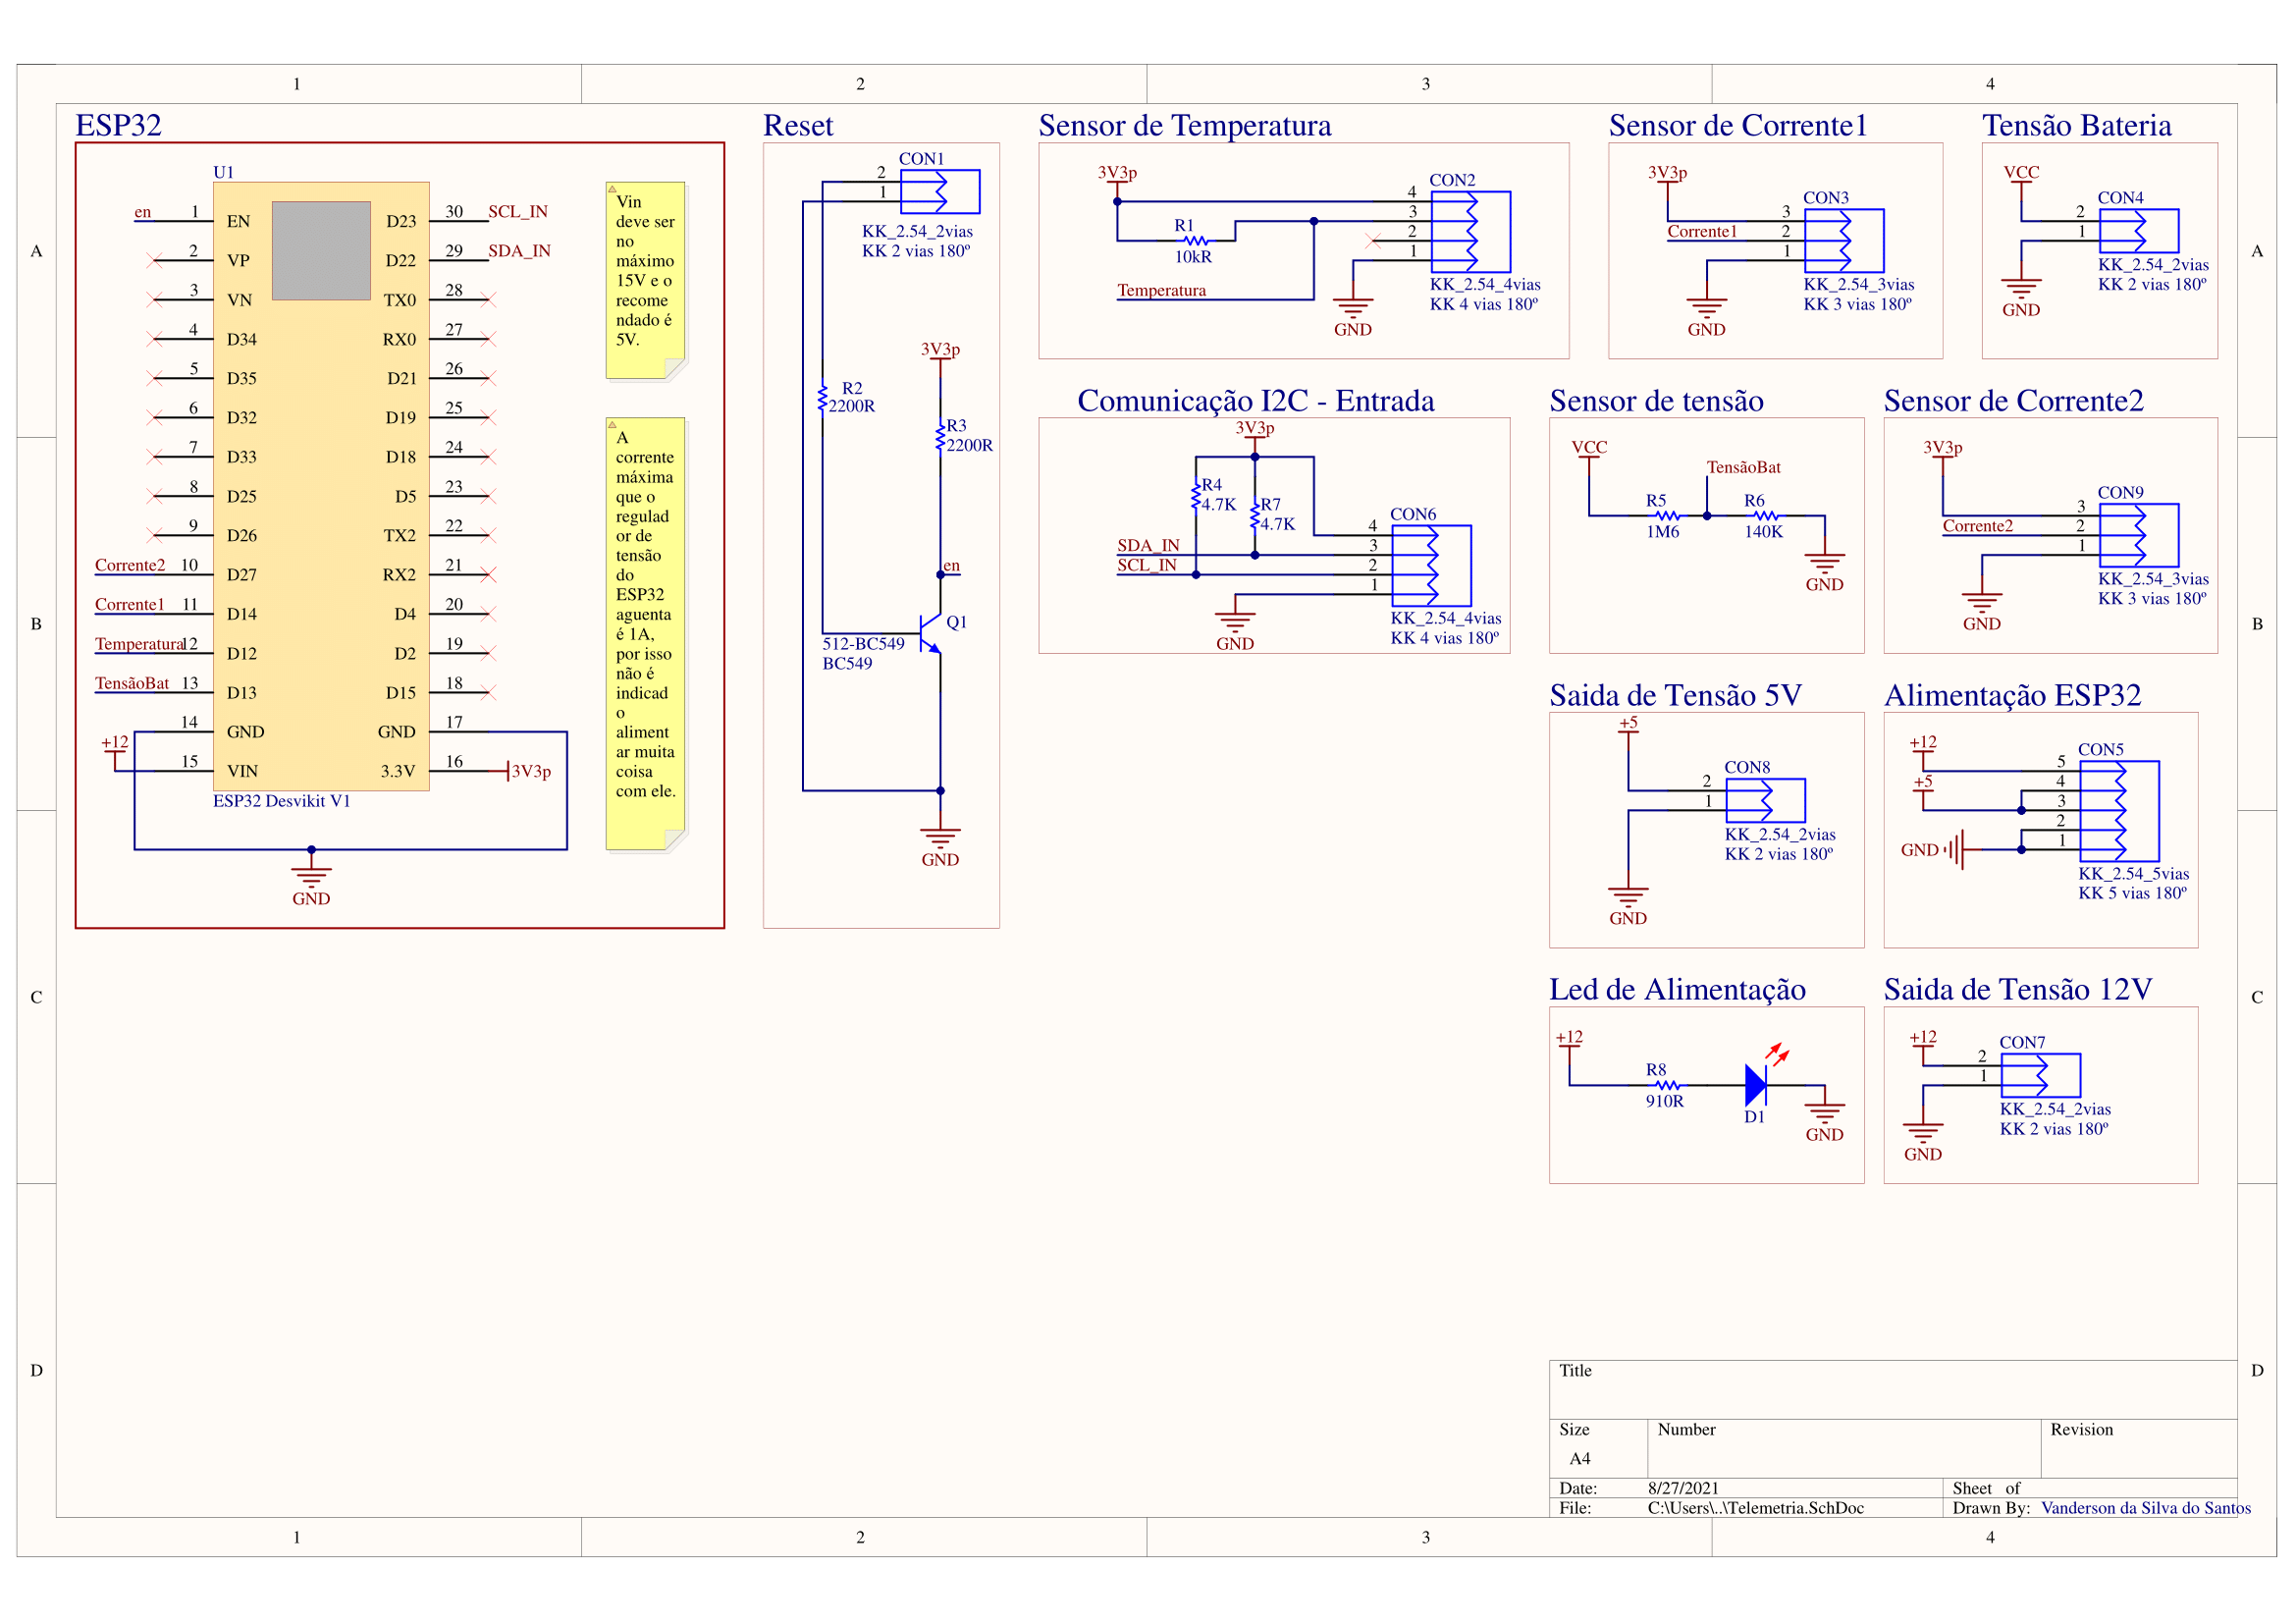
\includegraphics[width=17cm]{modulos/Telemetria-1.png}
    \caption*{Fonte: Elaborado pelo autor no software Altium Design\cite{altium21} }
    \label{Protótipo placa de ## - Esquemático principal}
\end{figure}

Para design do hardware do módulo de Telemetria foi utilizado o CAD e software Altium Designer 21 \cite{altium21} a partir de uma licença estudantil. O projeto completo está disponibilizado em \cite{github_modulos} e todos os componentes usado nesse protótipo podem ser visto na tabela ~\ref{table:Componentes Utilizados na placa de Telemetria - Protótipo}.

\begin{table}[!h]
\caption{Componentes Utilizados na placa de Telemetria - Protótipo}
\centering
\begin{adjustbox}{width=\columnwidth,center}
\begin{tabular}{|c|c|c|c|c|}
\hline
Component                   & Description                                    & Designator               & Footprint                   & Quantity \\ \hline
KK\_2.54\_2vias             & Conector KK 2.54mm 2   vias                    & CON1, CON4, CON7,   CON8 & KK\_2VIAS\_180º             & 4        \\ \hline
KK\_2.54\_4vias             & Conector KK 2.54mm 4   vias                    & CON2, CON6               & KK\_4vias\_180°             & 2        \\ \hline
KK\_2.54\_3vias             & Conector KK 2.54mm 3   vias                    & CON3, CON9               & KK\_3vias\_180º             & 2        \\ \hline
KK\_2.54\_5vias             & Conector KK 2.54mm 5   vias                    & CON5                     & KK\_5vias\_180°             & 1        \\ \hline
LED 5MM RED                 & LED 5MM RED                                    & D1                       & LED 5MM RED                 & 1        \\ \hline
BC549                       & TRANS NPN 30V 0.1A   TO-92                     & Q1                       & TO92                        & 1        \\ \hline
RES 470R 1/4W   CARBON FILM & RES 470R OHM 1/4W 5\%   CARBON FILM            & R1, R2, R3, R8           & RES 470R 1/4W CARBON   FILM & 4        \\ \hline
4.7K                        & RES 4.7K OHM 1/4W 5\%   CARBON FILM            & R4, R7                   & RES 4.7K 1/4W CARBON   FILM & 2        \\ \hline
1M6                         & RES 1.6M OHM                                   & R5                       & RESISTOR 0603               & 1        \\ \hline
140K                        & RES 140k OHM                                   & R6                       & RESISTOR 0805               & 1        \\ \hline
microcontrolador            & microcontrolador com   moculo bluethoth e wifi & U1                       & ESP32\_Desvikit\_v1         & 1        \\ \hline

\end{tabular}
\end{adjustbox}
\centering
\caption*{Fonte: Elaborado pelo autor}
\label{table:Componentes Utilizados na placa de Telemetria - Protótipo}
\end{table}

Dentre os componentes usados, nenhum muito diferente foi utilizado. Para mensurar a tensão, somente um divisor de tensão foi usado. Além disso, como já mencionado antes, também usamos o ESP32 \cite{esp32} como microcontrolador do módulo.

%------------------------------------------
\begin{wrapfigure}{r}{5.5cm}
\centering
\caption{ Sensor de temperatura e umidade dht 22}\label{wrap-fig:1}
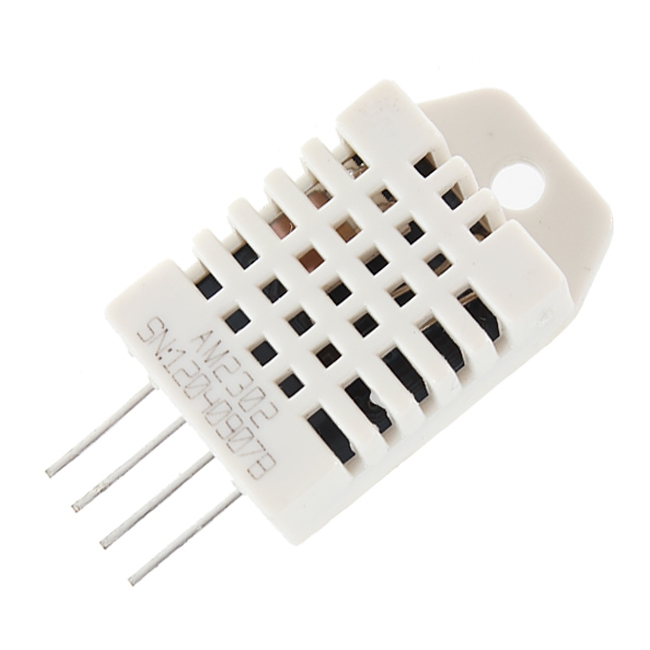
\includegraphics[width=4cm]{modulos/dht22_sensor.jpg}
\caption*{Fonte: Foto disponibilizada por botnroll}\label{wrap-fig:1}
\end{wrapfigure} 
%------------------------------------------

Para medir a temperatura e umidade dentro do robô foi usado o sensor DHT22 \cite{dht22_datasheet} e o sensor de corrente linear ACS712 \cite{ACS712_datasheet}. Sensores, como o de bateria, foram feitos na com resistores e capacitores.

\begin{figure}[!h]
    \centering
    \begin{minipage}{0.5\textwidth}
        \centering
        \caption{Protótipo Telemetria - PCB 2D}
        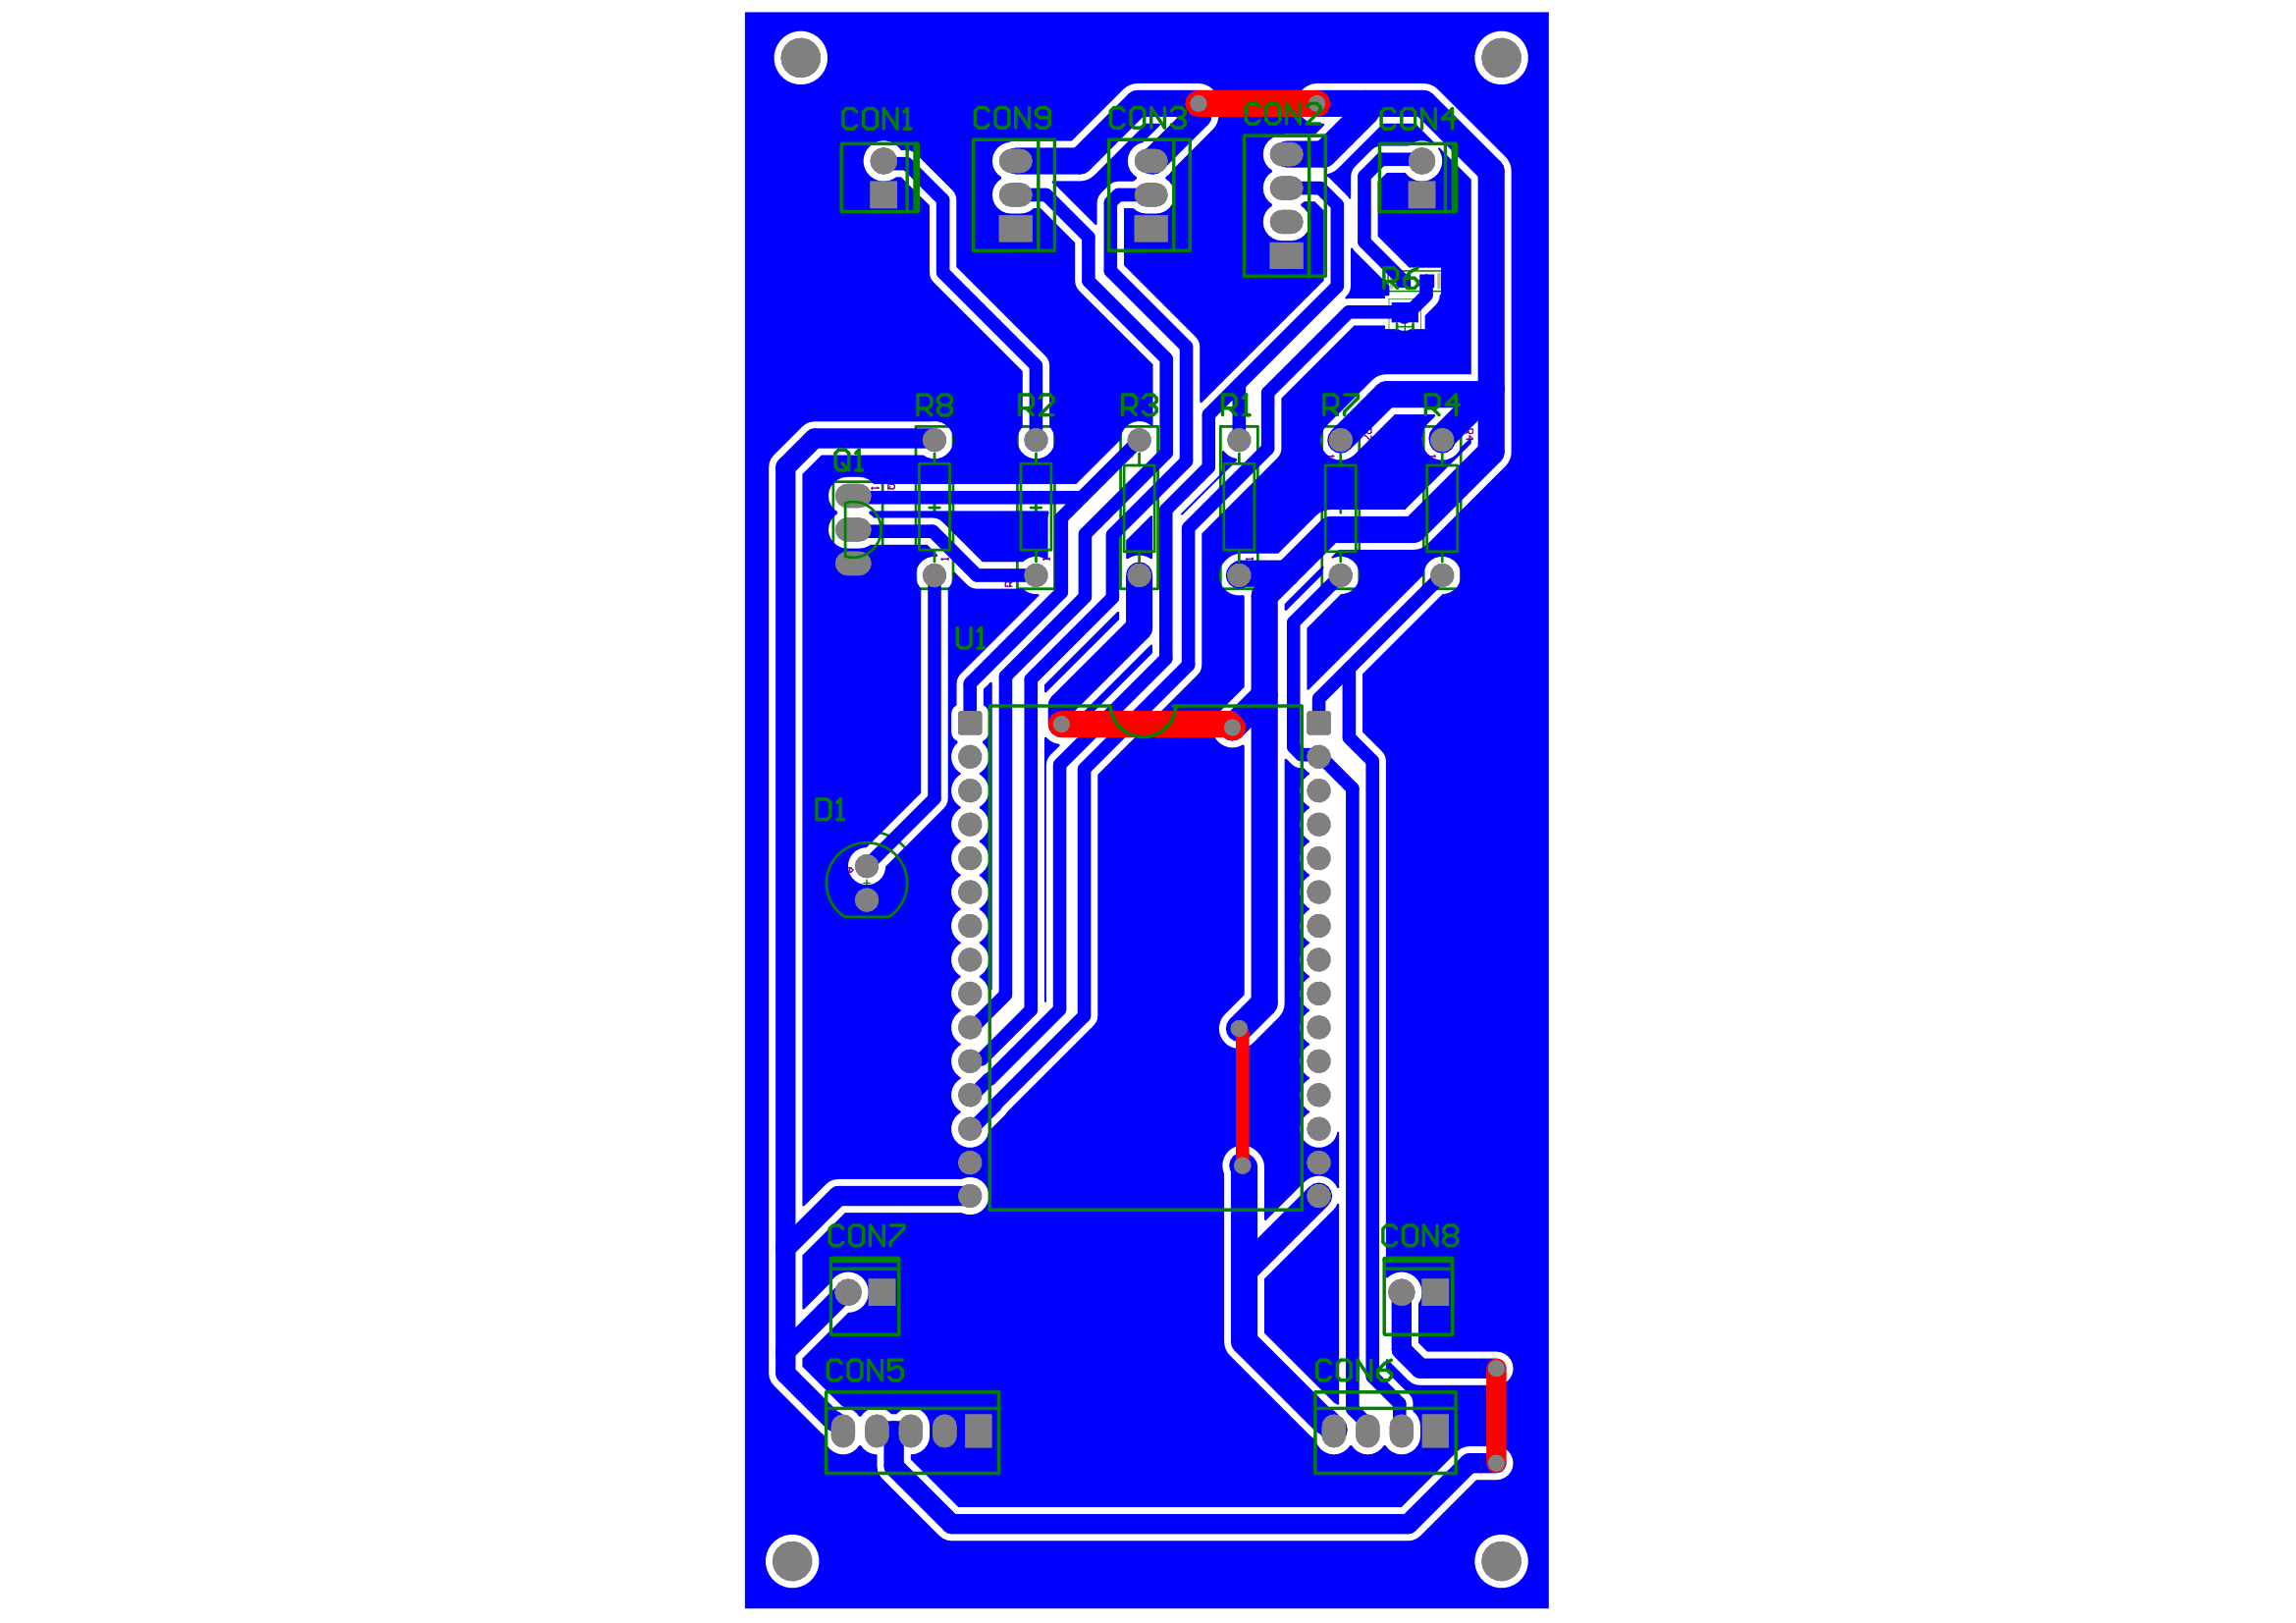
\includegraphics[width=1.03\textwidth]{modulos/Telemetria-2.png} 
        \label{Protótipo Telemetria - PCB 2D}
    \end{minipage}\hfill
    \begin{minipage}{0.5\textwidth}
        \centering
        \caption{Protótipo Telemetria - PCB 3D }
        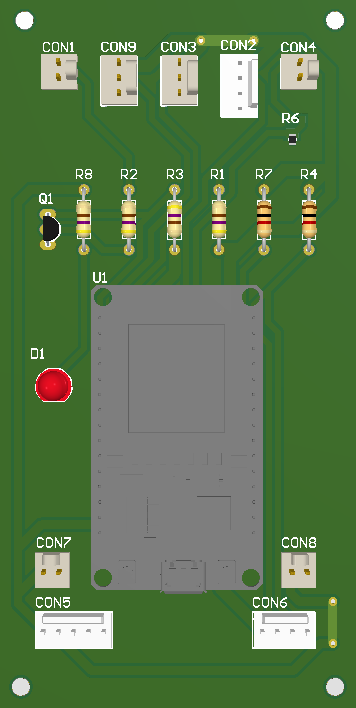
\includegraphics[width=0.4\textwidth]{modulos/Telemetria.png} 
        \label{Protótipo Telemetria - PCB 3D}
    \end{minipage}\hfill
    
    \caption*{Fonte: Elaborado pelo autor no software Altium Design\cite{altium21} }
    \label{fig:Protótipo Telemetria - PCB 2D3D}
\end{figure}

A partir do esquema elétrico que foi feito e do desenho da PCB, a placa de circuito impresso, em uma única camada (Single Layer) e dimensões de 120x60mm. As visões 2D e 3D podem ser vista na figura ~\ref{Protótipo Telemetria - PCB 2D} e ~\ref{Protótipo Telemetria - PCB 3D}.

\begin{comment}
\begin{figure}[!h]
    \centering
    \begin{minipage}{0.5\textwidth}
        \centering
        \caption{Protótipo Telemetria - Trilhas}
        \includegraphics[width=0.8\textwidth]{example-image-a} 
        \label{fig:figura1minipg}
    \end{minipage}\hfill
    \begin{minipage}{0.5\textwidth}
        \centering
        \caption{Protótipo Telemetria - Completa }
        \includegraphics[width=0.8\textwidth]{example-image-a} 
        \label{fig:figura1minipg}
    \end{minipage}\hfill
    
    \caption*{Fonte: Elaborado pelo autor }
    \label{fig:Protótipo Telemetria - TrilhasC}
\end{figure}
\end{comment}
%================================ TELEMETRIA OFICIAL ========================
\clearpage

\subsubsection{Oficial}

A placa oficial de Telemetria ainda não foi fabricada. Por se tratar de uma placa mais profissional, ela será mandada para ser feita para uma empresa privada ainda não escolhida, não na própria Universidade São Paulo. Assim como o protótipo, o projeto como um todo foi dividido em um esquemático e uma PCB.

\begin{figure}[!h]
\centering
    \caption{Placa de Telemetria - Esquemático principal }
    \centering % para centralizarmos a figura
    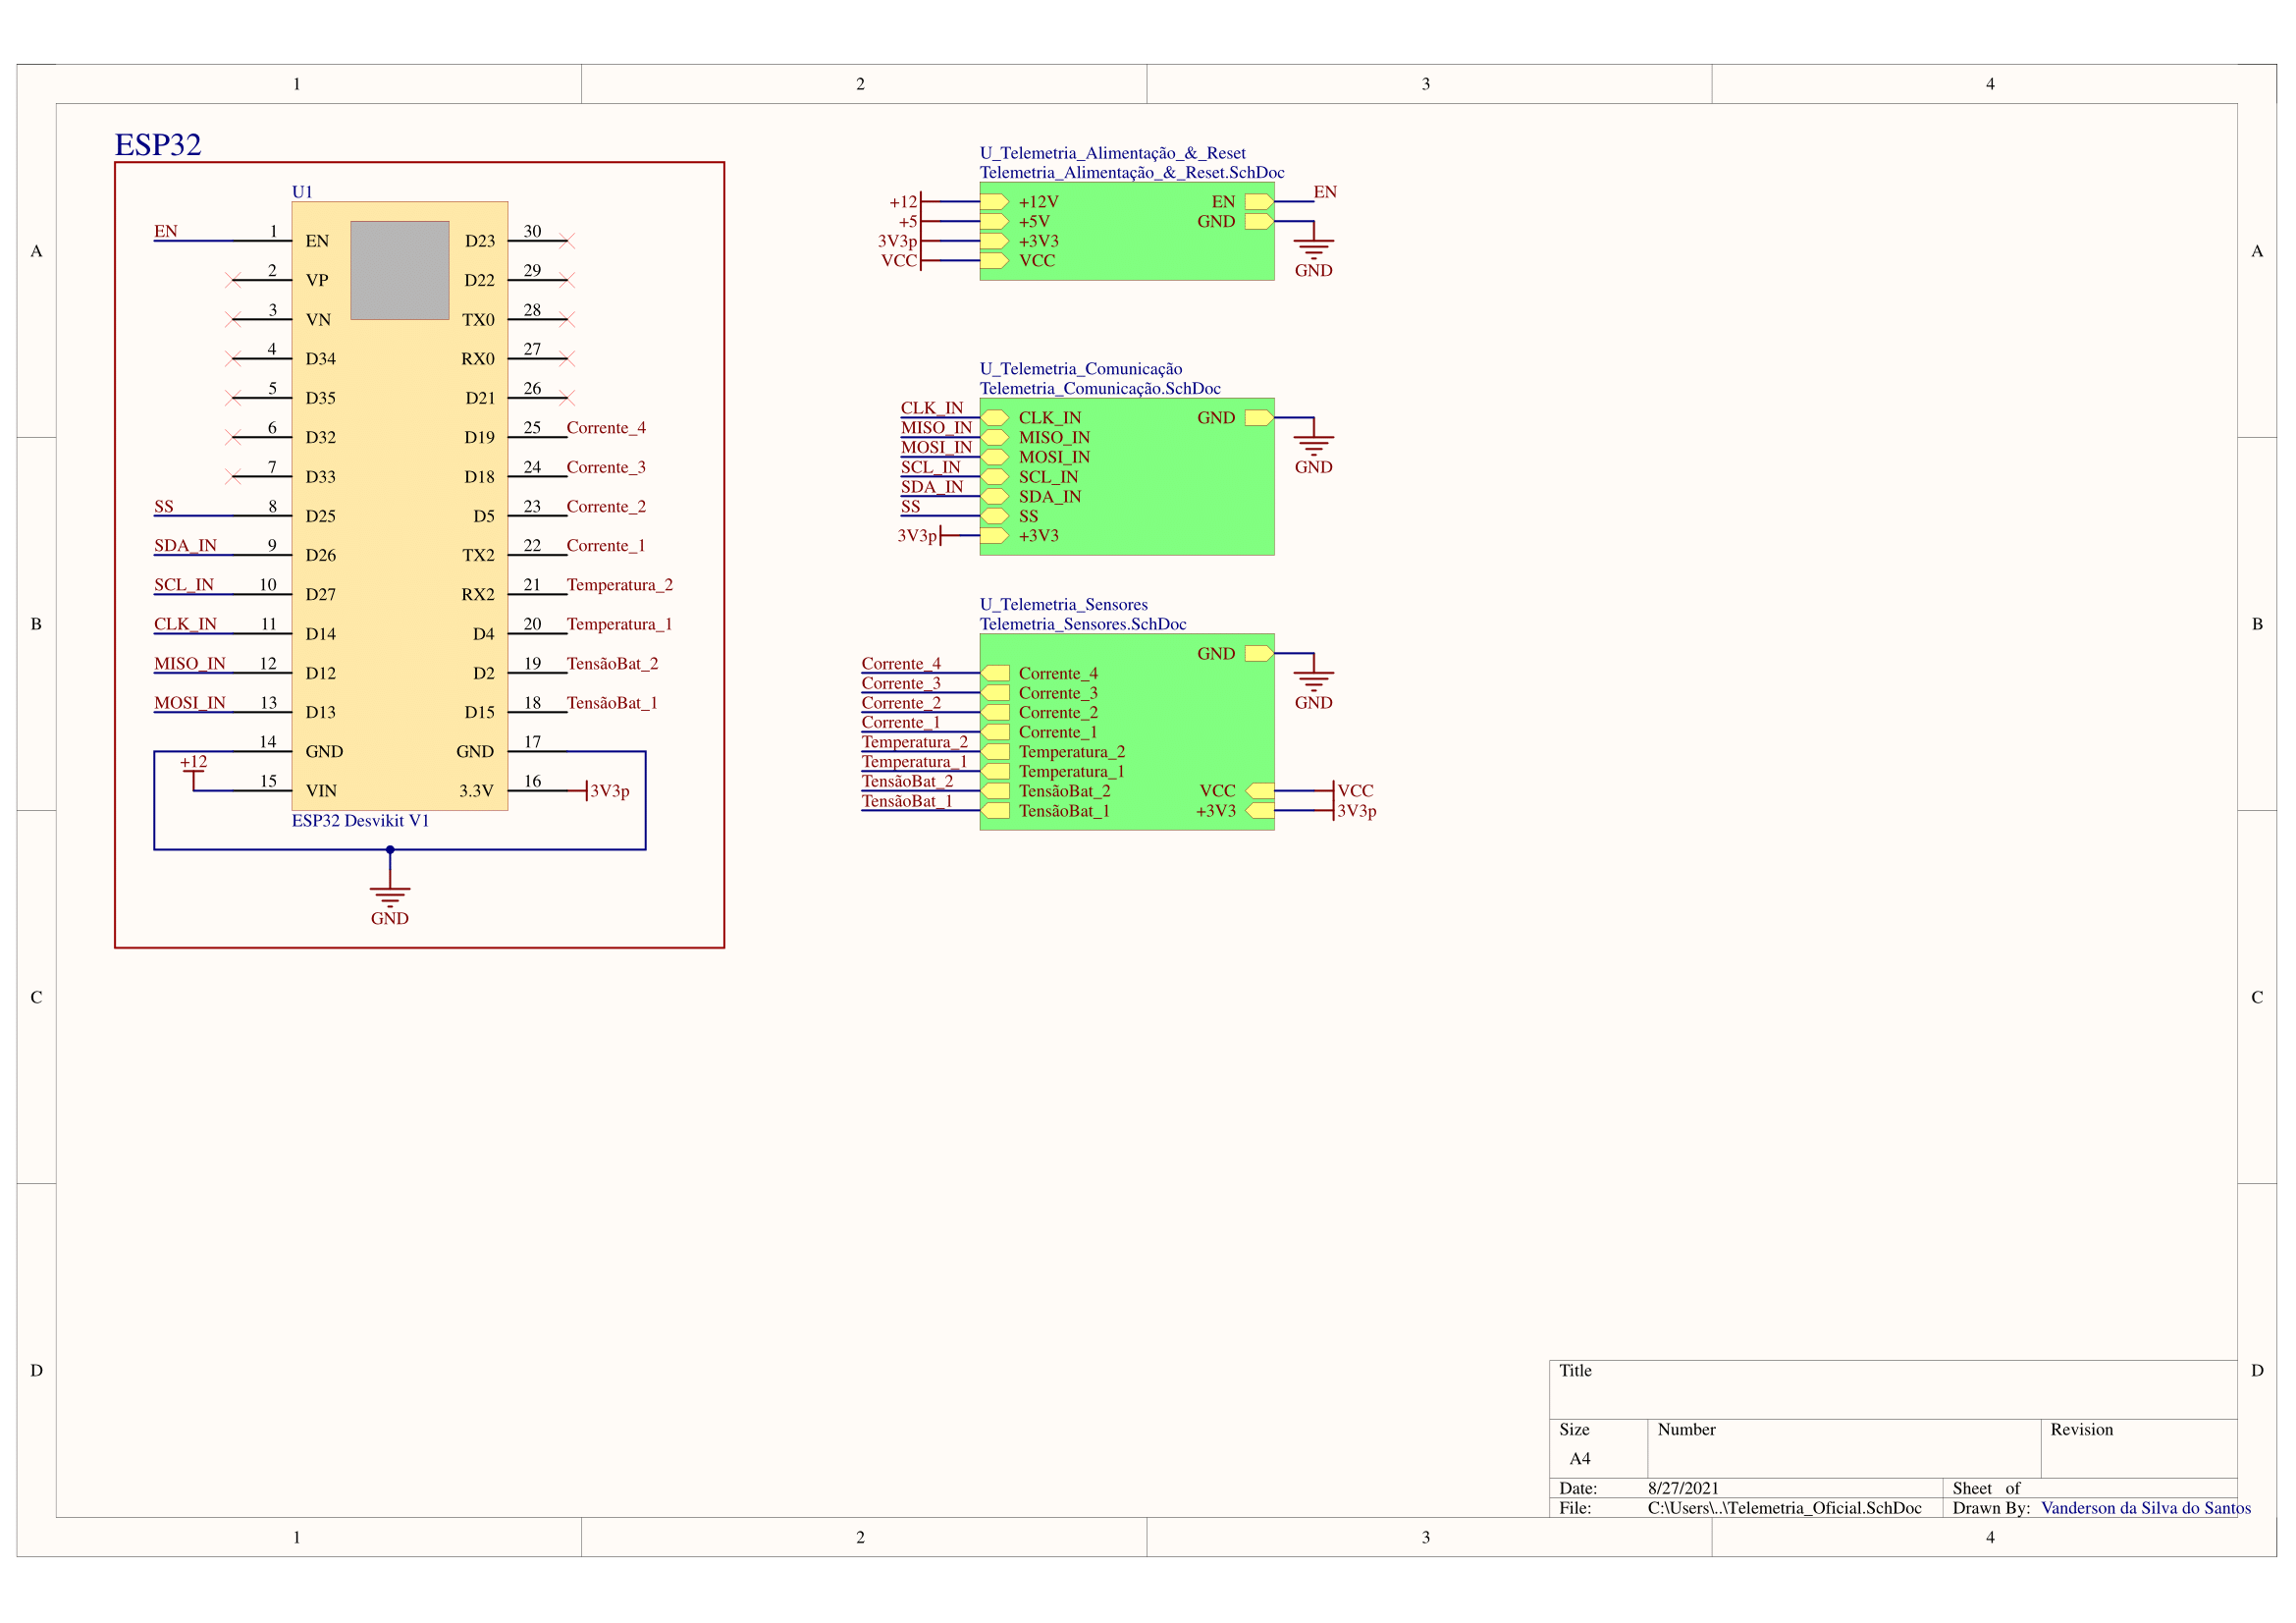
\includegraphics[width=17cm]{modulos/Telemetria_Oficial-1.png}
    \caption*{Fonte: Elaborado pelo autor no software Altium Design\cite{altium21} }
    \label{Protótipo placa de ## - Esquemático principal}
\end{figure}

Para design do hardware do módulo de Telemetria foi utilizado o CAD e software Altium Designer 21 \cite{altium21} a partir de uma licença estudantil. O projeto completo está disponibilizado em \cite{github_modulos} e todos os componentes usado nessa versão oficial podem ser visto na tabela ~\ref{table:Componentes Utilizados na placa de Telemetria}.

\begin{table}[!h]
\caption{Componentes Utilizados na placa de Telemetria}
\centering
\begin{adjustbox}{width=\columnwidth,center}
\begin{tabular}{|c|c|c|c|c|}

\hline
Component        & Description                                    & Designator                  & Footprint           & Quantity \\ \hline
KK\_2.54\_2vias  & Conector KK 2.54mm 2   vias                    & CON1, CON3, CON4,   CON5    & KK\_2VIAS\_180º     & 4        \\ \hline
KK\_2.54\_6vias  & Conector KK 2.54mm 6   vias                    & CON2                        & KK\_6vias\_180°     & 1        \\ \hline
KK\_2.54\_5vias  & Conector KK 2.54mm 5   vias                    & CON6                        & KK\_5vias\_180°     & 1        \\ \hline
KK\_2.54\_4vias  & Conector KK 2.54mm 4   vias                    & CON7, CON8, CON11           & KK\_4vias\_180°     & 3        \\ \hline
KK\_2.54\_3vias  & Conector KK 2.54mm 3   vias                    & CON9, CON10, CON12,   CON13 & KK\_3vias\_180º     & 4        \\ \hline
LED 3MM RED      & LED 3MM RED                                    & D1                          & LED RED             & 1        \\ \hline
Trans BC817      & Transistor BJT NPN   BC817-25-7-F              & Q1                          & SOT96P240X110-3N    & 1        \\ \hline
680R             & Resistor                                       & R1                          & RESC3216X60N        & 1        \\ \hline
2k2              & Resistor                                       & R2, R3                      & RESC3216X60N        & 2        \\ \hline
4k7              & Resistor                                       & R4, R5                      & RESC3216X60N        & 2        \\ \hline
10k              & Resistor                                       & R6, R7                      & RESC3216X60N        & 2        \\ \hline
1M6              & 0603                                           & R8, R10                     & RESISTOR 0603       & 2        \\ \hline
140K             & 0805                                           & R9, R11                     & RESISTOR 0805       & 2        \\ \hline
microcontrolador & microcontrolador com   moculo bluethoth e wifi & U1                          & ESP32\_Desvikit\_v1 & 1        \\ \hline

\end{tabular}
\end{adjustbox}
\centering
\caption*{Fonte: Elaborado pelo autor}
\label{table:Componentes Utilizados na placa de Telemetria}
\end{table}

Em relação ao protótipo, pouco mudou da lógica por trás do circuito, a principal diferença é que o modelo oficial utiliza todos componentes com encapsulamento SMD \cite{SMD_def}. Além disso, foi adicionado o protocolo de comunicação SPI também, como já foi comentado no início do capítulo.

\begin{figure}[!h]
    \centering
    \begin{minipage}{0.5\textwidth}
        \centering
        \caption{Telemetria - PCB 2D}
        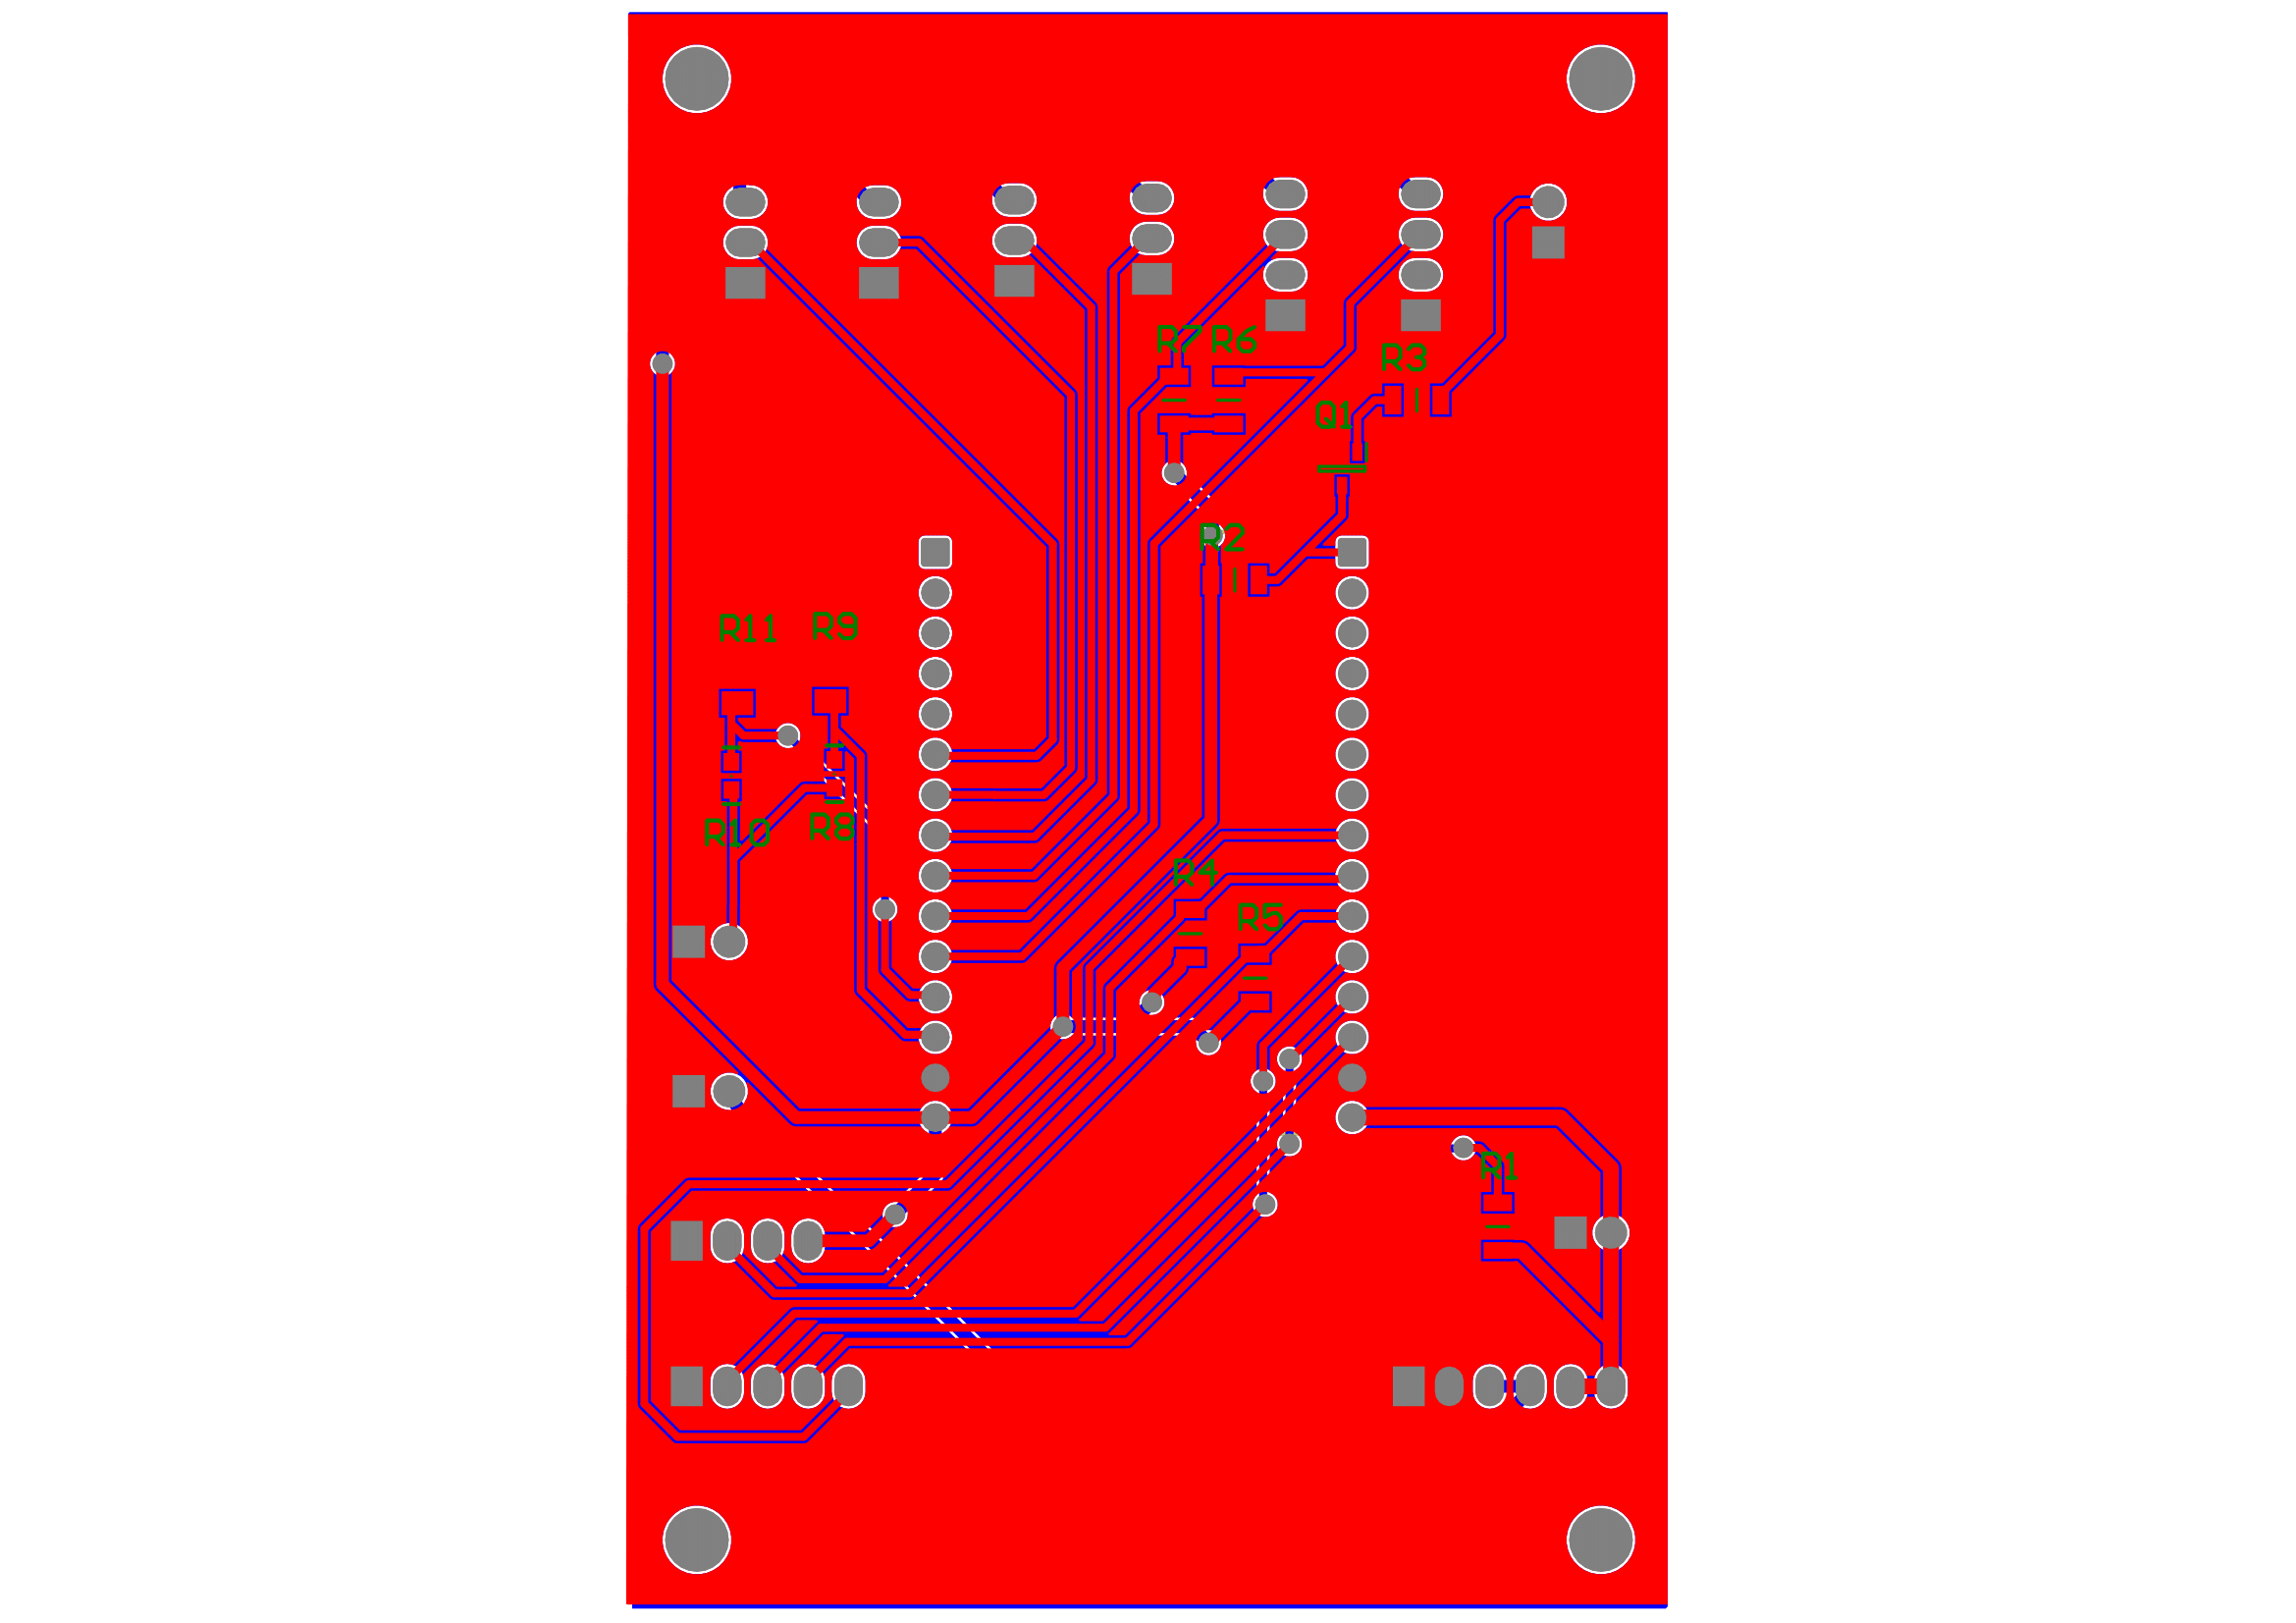
\includegraphics[width=1.03\textwidth]{modulos/Telemetria_Oficial-5.png} 
        \label{fig:figura1minipg}
    \end{minipage}\hfill
    \begin{minipage}{0.5\textwidth}
        \centering
        \caption{Telemetria - PCB 3D}
        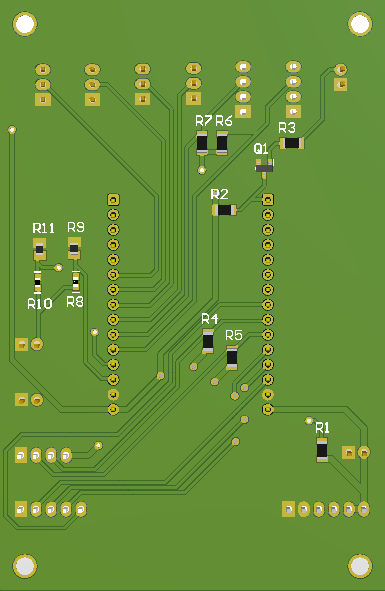
\includegraphics[width=0.5\textwidth]{modulos/Telemetria_Oficial.png} 
        \label{fig:figura1minipg}
    \end{minipage}\hfill
    
    \caption*{Fonte: Elaborado pelo autor no software Altium Design\cite{altium21} }
    \label{fig:figurasminipg}
\end{figure}

A placa de circuito impresso está completa, porém ainda não foi feito o pedido oficial de fabricação.

\begin{comment}
%================================ TELEMETRIA FIRMWARE ========================
\subsection{Firmware}
\end{comment}
\end{document}